\section{Containers}
\subsection{Übersicht}
\subsubsection{Sequence}
\begin{itemize}
	\item Reihenfolge bleibt erhalten
	\item find \chapref{find} in linearer Zeit
	\item array, vector, deque, list, forward\_list
\end{itemize}
\subsubsection{Associative}
\begin{itemize}
	\item Reihenfolge in sortierter Folge
	\item find \chapref{find} in logarithmischer Zeit
	\item map, multimap, set, multiset
\end{itemize}
\subsubsection{Hashed}
\begin{itemize}
	\item ohne Reihenfolge
	\item find \chapref{find} in konstanter Zeit
	\item unordered\_map, unordered\_multimap, \newline
		unordered\_set, unordered\_multiset
\end{itemize}
\subsubsection{Adaptors}
\begin{itemize}
	\item Provide a different interface for sequential containers. 
	\item stack
	\begin{itemize}
	\item limits to push / pop and top
	\item wraps deque, vector or list
	\end{itemize}
	\item queue
	\begin{itemize}
	\item push / pop / front
	\end{itemize}
	\item priority\_queue
	\begin{itemize}
	\item push / pop / top
	\item top() element is always smallest
	\end{itemize}
\end{itemize}
\subsection{Common API}
\begin{itemize}
	\item erease(iter)
	\item insert(iter,value)
	\item size(), empty()
	\item default-constructor
	\item copy-constructor
	\item equal-compare wenn Elemente gleicher Typ
	\item clear() $\rightarrow$ empty()
\end{itemize}
\subsubsection{Constructors}
	\begin{tabularx}{\columnwidth}{lX}
		Code & Bedeutung \\
		\hline
		C\{\} & Leerer Container besser als C() \\
		C\{e1,e2,\ldots,en\} & Mit \emph{initilizer list} initialisieren \\
		C\{n, e\} & Mit \emph{n} Kopien von \emph{e} initialisieren.  Besser C(n,e) verwenden, da sonst eine Mehrdeutigkeit ensteht, wenn \emph{n} ein gültiges Element des Containers ist (z.B. bei $vector<int>$) \\
		C\{ita, itb\} & Mit Elementen von iterator \emph{ita} bis ohne \emph{itb} initialisieren \\
	\end{tabularx}
	Beispiele:
\begin{lstlisting}
	std::vector<int> v{1,2,3,5,7,11};
	std::list<int>   l(5,42);
	std::deque<int>  q{v.begin(),v.end()};
\end{lstlisting}

\subsection{vector}
\begin{center}
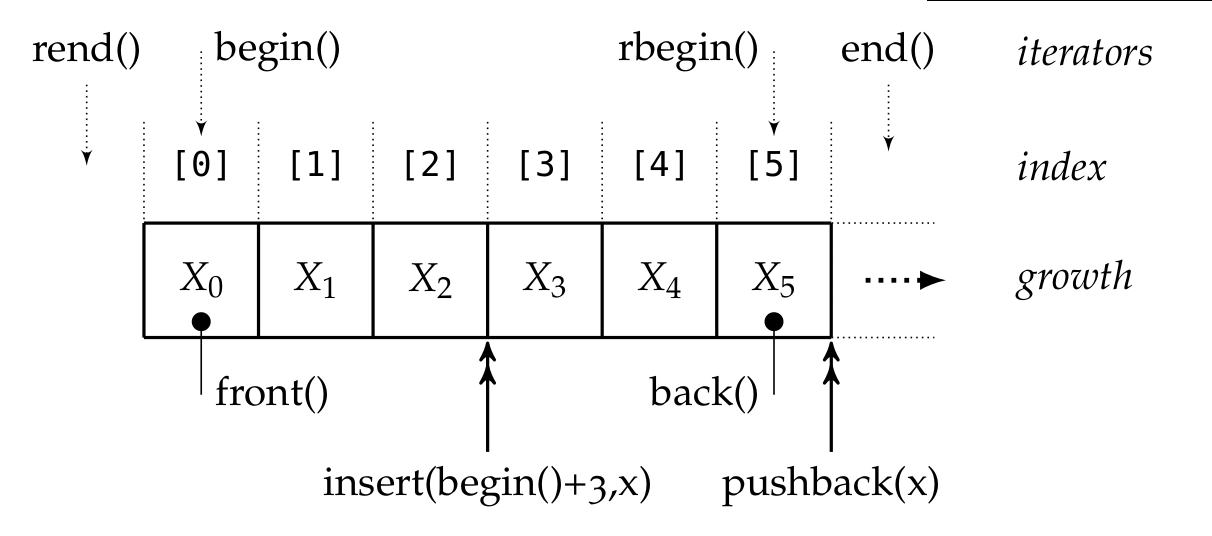
\includegraphics[width=\linewidth]{./bilder/iterators}
\end{center}
\begin{itemize}
\item Bool vector is bad because of premature optimization
\end{itemize}


\subsection{deque}
\begin{itemize}
\item push\_front / pop\_front
\end{itemize}

\subsection{array}
\begin{itemize}
\item similar to C-array (fixed size), but keeps size
\item initialization needs \{\{\}\}
\end{itemize}

\subsection{list}
\begin{itemize}
\item double linked list
\item fast insert in any position
\end{itemize}

\subsection{set}
\begin{itemize}
\item own member functions for find and count which are more efficient
\end{itemize}
\begin{lstlisting}
#include <set>
#include <iostream>
void filtervowels(std::istream &in, std::ostream &out){
	 std::set<char> const vowels{'a','e','o','u','i','y'};
	 char c{};
	 while (in>>c)
	 	 if (! vowels.count(c))
	 	 	 out << c;
}
int main(){
	 filtervowels(std::cin,std::cout);
}
\end{lstlisting}

\subsection{map}
\begin{lstlisting}
#include <map>
#include <iostream>
#include <iterator>
int main(){
	 std::map<char,size_t> vowels
	
{{'a',0},{'e',0},{'i',0},{'o',0},{'u',0},{'y',0}};
	 char c;
	 while (std::cin >> c)
	 	 if (vowels.count(c))
	 	 	 ++vowels[c];
	 for(auto const &p:vowels)
	 	 std::cout << p.first << " = "<< p.second << '\n';
}
\end{lstlisting}
